\documentclass{mimosis}

% \usepackage{metalogo}

\renewcommand{\floatpagefraction}{.8}%

\usepackage{chngcntr}
\counterwithout{figure}{chapter}
% \setcounter{tocdepth}{2}

%%%%%%%%%%%%%%%%%%%%%%%%%%%%%%%%%%%%%%%%%%%%%%%%%%%%%%%%%%%%%%%%%%%%%%%%
% Some of my favourite personal adjustments
%%%%%%%%%%%%%%%%%%%%%%%%%%%%%%%%%%%%%%%%%%%%%%%%%%%%%%%%%%%%%%%%%%%%%%%%
%
% These are the adjustments that I consider necessary for typesetting
% a nice thesis. However, they are *not* included in the template, as
% I do not want to force you to use them.

% This ensures that I am able to typeset bold font in table while still aligning the numbers
% correctly.
\usepackage{etoolbox}

\usepackage[binary-units=true]{siunitx}
% \DeclareSIUnit\px{px}
\DeclareSIUnit\parsec{pc}

\sisetup{%
  detect-all           = true,
  detect-family        = true,
  detect-mode          = true,
  detect-shape         = true,
  detect-weight        = true,
  detect-inline-weight = math,
}

%%%%%%%%%%%%%%%%%%%%%%%%%%%%%%%%%%%%%%%%%%%%%%%%%%%%%%%%%%%%%%%%%%%%%%%%
% Hyperlinks & bookmarks
%%%%%%%%%%%%%%%%%%%%%%%%%%%%%%%%%%%%%%%%%%%%%%%%%%%%%%%%%%%%%%%%%%%%%%%%

\usepackage[%
  colorlinks = true,
  citecolor  = RoyalBlue,
  linkcolor  = RoyalBlue,
  urlcolor   = RoyalBlue,
  ]{hyperref}

\addto\extrasenglish{%
  \renewcommand{\chapterautorefname}{Chapter}%
  \renewcommand{\figureautorefname}{Fig.}%
  \renewcommand{\equationautorefname}{Eq.}%
  \renewcommand{\sectionautorefname}{Section}%
  \renewcommand{\subsectionautorefname}{Section}%
}

\usepackage{bookmark}

%%%%%%%%%%%%%%%%%%%%%%%%%%%%%%%%%%%%%%%%%%%%%%%%%%%%%%%%%%%%%%%%%%%%%%%%
% Bibliography
%%%%%%%%%%%%%%%%%%%%%%%%%%%%%%%%%%%%%%%%%%%%%%%%%%%%%%%%%%%%%%%%%%%%%%%%
%
% I like the bibliography to be extremely plain, showing only a numeric
% identifier and citing everything in simple brackets. The first names,
% if present, will be initialized. DOIs and URLs will be preserved.

% \usepackage[%
%   % autocite     = plain,
%   % backend      = bibtex,
%   doi          = true,
%   url          = true,
%   giveninits   = true,
%   hyperref     = true,
%   maxbibnames  = 99,
%   maxcitenames = 99,
%   % sortcites    = true,
%   style        = apa,
%   % citestyle    = authoryear,
%   % autocite     = inline,
%   backend      = biber,
%   natbib       = true,
%   ]{biblatex}

\usepackage[utf8]{inputenc}

\usepackage[
    backend      = biber,
    style        = authoryear,
    hyperref     = true,
    natbib       = true,
    maxcitenames = 2,
    bibencoding  = utf8,
    dashed       = false,
    doi         = false,
    % eprint      = false,
]{biblatex}

\renewbibmacro{in:}{}
\def\apj{ApJ}  
\def\apjl{Astrophys. J. Lett.}
\def\apjs{Astrophys. J. Supp.}
\def\mnras{Mon.Not.Roy.As.Soc.}
\def\araa{Annu. Rev. Astron. Astrophys.}
\def\aj{Astron. J.}
\def\asap{Astron. Astrophys.}
\def\aap{Astron. \& Astrophys.}
\def\prd{Phys.~Rev.~D}
\def\nat{Nature}
\def\jcap{J. Cosmology Astropart. Phys.}

% \input{bibliography-mimosis}
% \bibliographystyle{ieeetr}
% \bibliographystyle{kp}

% llibrary: nasa ads
% library2: google scholar cites with authors from nasa ads
% library3: google scholar cites
\bibliography{library2}
% \addbibresource{library.bib}

%%%%%%%%%%%%%%%%%%%%%%%%%%%%%%%%%%%%%%%%%%%%%%%%%%%%%%%%%%%%%%%%%%%%%%%%
% Fonts
%%%%%%%%%%%%%%%%%%%%%%%%%%%%%%%%%%%%%%%%%%%%%%%%%%%%%%%%%%%%%%%%%%%%%%%%

\ifxetexorluatex
  \setmainfont{Minion Pro}
\else
  \usepackage[lf]{ebgaramond}
  % \usepackage{palatino}
  % \usepackage{ebgaramond}
  \usepackage[oldstyle,scale=0.7]{sourcecodepro}
  \singlespacing
\fi

\renewcommand{\th}{\textsuperscript{\textup{th}}\xspace}

%%%%%%%%%%%%%%%%%%%%%%%%%%%%%%%%%%%%%%%%%%%%%%%%%%%%%%%%%%%%%%%%%%%%%%%%
% Incipit
%%%%%%%%%%%%%%%%%%%%%%%%%%%%%%%%%%%%%%%%%%%%%%%%%%%%%%%%%%%%%%%%%%%%%%%%

\title{The role of the cosmological constant in gravitational lensing}
\author{CID: 00919977}

% \linespread{1.15}
\linespread{1.25}
% \usepackage{layouts}

\begin{document}

% \printinunitsof{mm}{\pagevalues}
% \pagediagram

\frontmatter
  
%!TEX root = ../thesis.tex
\begin{titlepage}

\vspace*{2cm}
\makeatletter
\center
%----------------------------------------------------------------------------------------
%   HEADING SECTIONS
%----------------------------------------------------------------------------------------

\textsc{\Large Imperial College London}\\[0.2cm] 
\textsc{\large Department of Physics}\\[0.5cm] 

\vspace*{2cm}

\begin{Huge}
  \@title
\end{Huge}\\[0.1cm]
%
% \begin{Large}
%   \@subtitle
% \end{Large}\\
%
\emph{by}\\
\@author\\
%
\vspace*{3cm}
% \begin{minipage}{0.4\textwidth}
% \begin{flushright} \large

Project code: ASTR-Heavens-1\\
Supervisor: Prof. Alan \textsc{Heavens} \\ % Supervisor's Name
Assessor: Prof. Carlo \textsc{Contaldi} \\
Word count: 8256
% \end{flushright}
% \end{minipage}\\[4cm]

% \vfill
% A document submitted in partial fulfillment
% of the requirements for the degree of\\
% \emph{Technical Report}\\
% at\\
% \textsc{Miskatonic University}

\makeatother


\end{titlepage}

\newpage
\null
\thispagestyle{empty}
\newpage
  %!TEX root = ../thesis.tex
\begin{center}
  \LARGE Acknowledgements
\end{center}
%
\noindent
%

% \chapter*{Acknowledgements}

I wish to thank my supervisor Prof. Alan Heavens for his guidance and support through this project. I would also like to extend special thanks to Pierre Fleury, whom I've never met, for writing the paper that clearly laid out some of the important mathematics to get me started on light propagation in the Swiss-Cheese, without whom I would have been stuck for much longer. 
  %!TEX root = ../thesis.tex
\addcontentsline{toc}{chapter}{Abstract}

\begin{abstract}

Text of the Abstract.

\end{abstract}

  \tableofcontents

\mainmatter

  %!TEX root = ../thesis.tex
\chapter{Introduction}

There has been a debate over the past decade about whether the cosmological constant enters directly into the gravitational lensing equation. 

\section{Previous work}
% The conventional view \cite{islam1983cosmological} states that the cosmological constant does not directly play a role in gravitational lensing, \cite{simpson2010lensing} apart from 

% notation
\section{A note on units and notation}
I use a comma to denote partial derivative and an overdot to denote derivative with respect to the affine parameter $\lambda$. For example, $x_{,t}$ refers to $\frac{\partial x}{\partial t}$ and $\dot{x} = \frac{dx}{d\lambda}$. Throughout this work I use natural units such that $c = G = 1$. 

\section{Background}

In General Relativity, spacetime is described by a metric tensor $g$. 

The Einstein field equations (EFE) 

This is the analogue of Poisson's equation in Newtonian gravity. 

The motion of a partice is described by a trajectory $x^{\mu}(\lambda)$

Objects move on a geodesic, which is a generalisation of the notion of "straight lines" to a curved spacetime. The equations can be derived 

The geodesic equation is 

\begin{equation}
  \ddot{x}^{\mu} + \Gamma^{\mu}_{\alpha \beta} \dot{x}^{\alpha} \dot{x}^{\beta} = 0 
  \label{eq:geodesic-eqn}
\end{equation}

where an overdot represents a derivative with respect to the affine parameter $\lambda$, and $\Gamma$ are the Christoffel symbols given by

\begin{equation}
  \Gamma^{\mu}_{\alpha \beta} = \frac{1}{2} g^{\mu \rho} (g_{\rho \alpha, \beta} + g_{\rho \beta, \alpha} - g_{\alpha \beta, \rho}).
  \label{eq:christoffels}
\end{equation}

\begin{equation}
  g_{\mu \nu} dx^{\mu} dx^{\nu}
  \label{eq:null-condition}
\end{equation}

% EL equations
  %!TEX root = ../thesis.tex
\chapter{Gravitational lensing formalism}
\label{chapter:gravitational-lensing-formalism}

\section{Mathematical preliminaries}

The essence of General Relativity (GR) is very elegantly summarised by John Wheeler \citep[pg.235]{wheeler2000geons} in a sentence: matter tells spacetime how to curve, and spacetime tells matter how to move. 

The first half of this statement is quantified by the Einstein Field Equations (EFEs), which is the analogue of Poisson's equation in Newtonian gravity. They are a group of 10 coupled differential equations that describe the interaction between matter and geometry of spacetime, given by (in tensor notation)

\begin{equation}
  G_{\mu \nu} + \Lambda g_{\mu \nu} = 8\pi T_{\mu \nu}
  \label{eq:efes}
\end{equation}
where $g_{\mu \nu}$ is the metric of spacetime, $\Lambda$ is the cosmological constant, $G_{\mu \nu}$ is the Einstein tensor and $T_{\mu \nu}$ is the energy-momentum tensor. The energy momentum tensor on the right hand side is a source term that encodes how matter is distributed in the universe, and on the left hand side the Einstein tensor depends on the metric tensor, which describes the spacetime geometry. For a perfect pressureless fluid, the energy momentum tensor is

\begin{equation}
  T^{\mu \nu} = \rho u^{\mu} u^{\nu}
\end{equation}
where $u^{\mu}$ is the 4-velocity of the fluid. 

If we solve Einstein's field equations, we can obtain the metric tensor $g_{\mu \nu}$, which encodes the spacetime geometry. The metric tensor then influences how a particle behaves in this spacetime, bringing us to the second part of the statement: spacetime tells matter how to move. Given a metric tensor $g_{\mu \nu}$, we can first write down the line element

\begin{equation}
  ds^2 = g_{\mu \nu} dx^{\mu} dx^{\mu}
  \label{eq:line-element}
\end{equation}

Equations of motion of a particle moving in this spacetime can then be derived by first considering the Lagrangian of this particle

\begin{equation}
  \mathcal{L} = \sqrt{g_{\mu \nu} \frac{dx^{\mu}}{d \lambda} \frac{dx^{\nu}}{d \lambda}}
\end{equation}
where $\lambda$ is an affine parameter which increases monotonically along the particle's worldline and $x^{\mu}(\lambda)$ describes the trajectory of the particle. Between two spacetime points $A$ and $B$, we want to maximize $\int^{A}_{B} L(x^{\mu}, \dot{x}^{\mu})\, d \lambda$, so $\mathcal{L}$ satisfies the Euler-Lagrange (E-L) equations

\begin{equation}
  \frac{\partial \mathcal{L}}{\partial x^{\mu}} - \frac{d}{d \lambda}\left ( \frac{\partial \mathcal{L}}{\partial \dot{x}^{\mu}} \right ) = 0.
  \label{eq:euler-lagrange-eqn}
\end{equation}

From the E-L equations we arrive at the geodesic equation

\begin{equation}
  \ddot{x}^{\mu} + \Gamma^{\mu}_{\alpha \beta} \dot{x}^{\alpha} \dot{x}^{\beta} = 0 
  \label{eq:geodesic-eqn}
\end{equation}
where an overdot represents a derivative with respect to the affine parameter $\lambda$, and $\Gamma$ are the Christoffel symbols given by

\begin{equation}
  \Gamma^{\mu}_{\alpha \beta} = \frac{1}{2} g^{\mu \rho} (g_{\rho \alpha, \beta} + g_{\rho \beta, \alpha} - g_{\alpha \beta, \rho}).
  \label{eq:christoffels}
\end{equation}

A freely moving particle always moves along a geodesic, which is a generalisation of the notion of "straight lines" to a curved spacetime. In addition, light, as a massless particle, travels along null geodesics, in contrast to timelike ones for massive particles. Therefore, all light trajectories have to satisfy the null condition

\begin{equation}
  g_{\mu \nu} dx^{\mu} dx^{\nu} = 0.
  \label{eq:null-condition}
\end{equation}

The result is a handful of coupled differential equations that need to be solved to find the trajectory of light. Nevertheless, a common problem arising in cosmology stems from the fact that as soon as we depart from the simplest homogeneous models used by observational cosmologists, the task of finding solutions to null geodesics quickly becomes an intractable analytical problem. In our work, we instead use a numerical method to integrate the null geodesics to find the trajectory of the photon. 

\section{Derivation of bending angle in the Schwarzschild metric}

It is useful to first revise gravitational lensing in a universe without $\Lambda$, in a Schwarzschild metric, which is well understood. This will form the basis for our comparison with a universe that includes $\Lambda$. 

Spacetime outside a spherically symmetric distribution of matter and vacuum everywhere else is described by the Schwarzschild metric, one of the first known solutions to Einstein's field equations. Its line element is given by

\begin{equation}
  ds^2 = -\left ( 1- \frac{2M}{r} \right ) dt^2 + \left ( 1 - \frac{2M}{r}\right )^{-1} dr^2 + r^2(d\theta^2 + \sin^2\theta d \phi^2).
  \label{eq:schwarzschild-metric}
\end{equation}
where $M$ is the central mass. 

Due to spherical symmetry, we can restrict ourselves to the equatorial plane $\theta = \pi/2$ without loss of generality. This metric is asymptotically flat as $r \rightarrow \infty$. We can then find the total deflection angle $\alpha$ experienced by light that comes in from $r=-\infty$, gets deflected, and travels on towards $r=+\infty$ as 

\begin{equation}
  \alpha = 2 \int_{r_0}^{\infty} \left |  \frac{d\phi}{dr} \right | dr - \pi
\end{equation}
where $r_0$ is the distance of closest approach. 

The static nature and spherical symmetry of the Schwarzschild metric implies that there are two constants of motion for any particle traveling in this geometry. These can be obtained through direct application of the E-L equation (\autoref{eq:euler-lagrange-eqn}), and we have

\begin{subequations}
  \begin{align}
    E &= \left ( 1 - \frac{2M}{r} \right ) \dot{t},\\
    L &= r^2\dot{\phi}.
  \end{align}
  \label{eq:schwarzschild-constants}
\end{subequations}

By applying the null condition (\autoref{eq:null-condition}) on the metric, we obtain an expression for $\frac{d\phi}{dr}$

\begin{equation}
  \frac{d\phi}{dr} = \pm \frac{1}{r^2} \sqrt{\frac{1}{ \frac{1}{b^2} - \left (1- \frac{2M}{r} \right )\frac{1}{r^2} }}
  \label{eq:dphi-dr}
\end{equation}
where $b = L/E$ is the impact parameter (since $\frac{d\phi}{dr} = \dot{\phi}/\dot{r}$). Integrating this (for a detailed derivation see \cite{keeton2005formalism}), we obtain an expression for the bending angle $\alpha$ as a series expansion in $M/r_0$. This series, to third order in $M/r_0$, is as follows:

\begin{equation}
  \alpha = 4 \frac{M}{r_0} + \left ( -4 + \frac{15\pi}{4} \right )\left ( \frac{M}{r_0}\right )^2 + \left ( \frac{122}{3} - \frac{15\pi}{2} \right )\left ( \frac{M}{b}\right )^2.
  \label{eq:lensing-series-expansion-r0}
\end{equation}

This can be easily converted to a series in $M/b$ instead of $M/r_0$, which is usually done in literature, since a relation between $b$ and $r_0$ can be derived in a series expansion by setting $\dot{r} = 0$, giving \citep{keeton2005formalism}

\begin{equation}
  r_0 = b \left [ 1 - \frac{M}{b} - \frac{3}{2} \left ( \frac{M}{b}\right)^2 - 4\left ( \frac{M}{b}\right)^3 \right ].
  \label{eq:b-r0-relation}
\end{equation} 

This relation can then be used to rewrite the expansion in terms of $\frac{M}{b}$ to give us

\begin{equation}
  \alpha = 4 \frac{M}{b} + \frac{15\pi}{4} \left ( \frac{M}{b} \right )^2 + \frac{128}{3} \left ( \frac{M}{b} \right )^3.
  \label{eq:series-expansion-b}
\end{equation}
and indeed many authors use the impact parameter to discuss the bending of light in Schwarzschild spacetime \citep{wald2010general,misner2017gravitation,butcher2016no}. However, it has been pointed out previously by other authors \citep{ishak2008new,hammad2013note,lebedev2013influence} that in the non-zero $\Lambda$ case, the definition of the impact parameter is no longer independent of $\Lambda$ and this definition becomes questionable as spacetime is no longer asymptotically flat. 

In this work we will use another constant of the motion for the non-zero $\Lambda$ case, and for consistency we will use that parameter here as well so that a fair comparison can be made, even though the Schwarzschild case does not include a cosmological constant.

We can define another constant of the motion $R_u$ which corresponds to the unperturbed trajectory of light (see \autoref{fig:lensing}), which is related to $r_0$ by (see Eq. 6 of \citet{ishak2008new} and Eq. 3 of \citet{butcher2016no}).

\begin{equation}
  \frac{1}{r_0} = \frac{1}{R_u} + \frac{M}{R_u^2} + \frac{3M^2}{16R_u^3}
  \label{eq:r0-R-relation}
\end{equation}
where I have added a subscript $u$ to differentiate it from the Kottler coordinate $R$ in the next chapter. Using this relation and applying it to \autoref{eq:lensing-series-expansion-r0}, we can get a series expansion in $M/R_u$, which, up to third order, is given by

\begin{equation}
  \alpha = 4 \frac{M}{R_u} + \frac{15\pi}{4} \left ( \frac{M}{R_u} \right )^2 + \frac{401}{12} \left ( \frac{M}{R_u} \right )^3.
  \label{eq:series-expansion-R}
\end{equation}

There are 3 length quantities that are typically used in Schwarzschild lensing: the distance of closest approach $r_0$, the impact parameter $b$, and the parameter of the unperturbed trajectory $R_u$. They are related to each other through \autoref{eq:b-r0-relation} and \autoref{eq:r0-R-relation}, and their related series expansions are respectively given by \autoref{eq:lensing-series-expansion-r0}, \autoref{eq:series-expansion-b} and \autoref{eq:series-expansion-R}. The coefficient of the leading order term is the same for all three but they differ on higher order terms in the series expansion. Many gravitational lensing anayses done on the Schwarzschild metric are only concerned with the leading order term, and hence use these three lengths somewhat interchangeably. But in this project we are interested in corrections at the second order or higher, and the distinction becomes important. In the subsequent section of the report, we will be using the series expansion in $M/R_u$ (\autoref{eq:series-expansion-R}). 

As mentioned previously, \citet{rindler2007contribution} proposed a different expression for $\alpha$. The expression was later refined for a Swiss-cheese universe \citep{ishak2008new}, and I will state it here (in our notation) for easy comparison:

\begin{equation}
  \alpha_{\text{Ishak}} = 4 \frac{M}{R_u} + \frac{15\pi}{4} \left ( \frac{M}{R_u} \right )^2 + \frac{305}{12} \left ( \frac{M}{R_u} \right )^3 - \frac{\Lambda R_u R_h}{3},
  \label{eq:rindler-ishak-alpha}
\end{equation}
where $R_h$ is the boundary of the hole in static coordinates in the Swiss-cheese model. The $\Lambda$-term is negative, and they postulate that the cosmological constant attenuates lensing. 

\section{Lensing observables}

A significant part of the conflict in literature comes from the question of which quantities in lensing are observable, and whether these observable quantities are ultimately affected by the presence of the cosmological constant. Therefore we aim to stick with strictly observable quantities. 

\begin{figure}
  \centering
  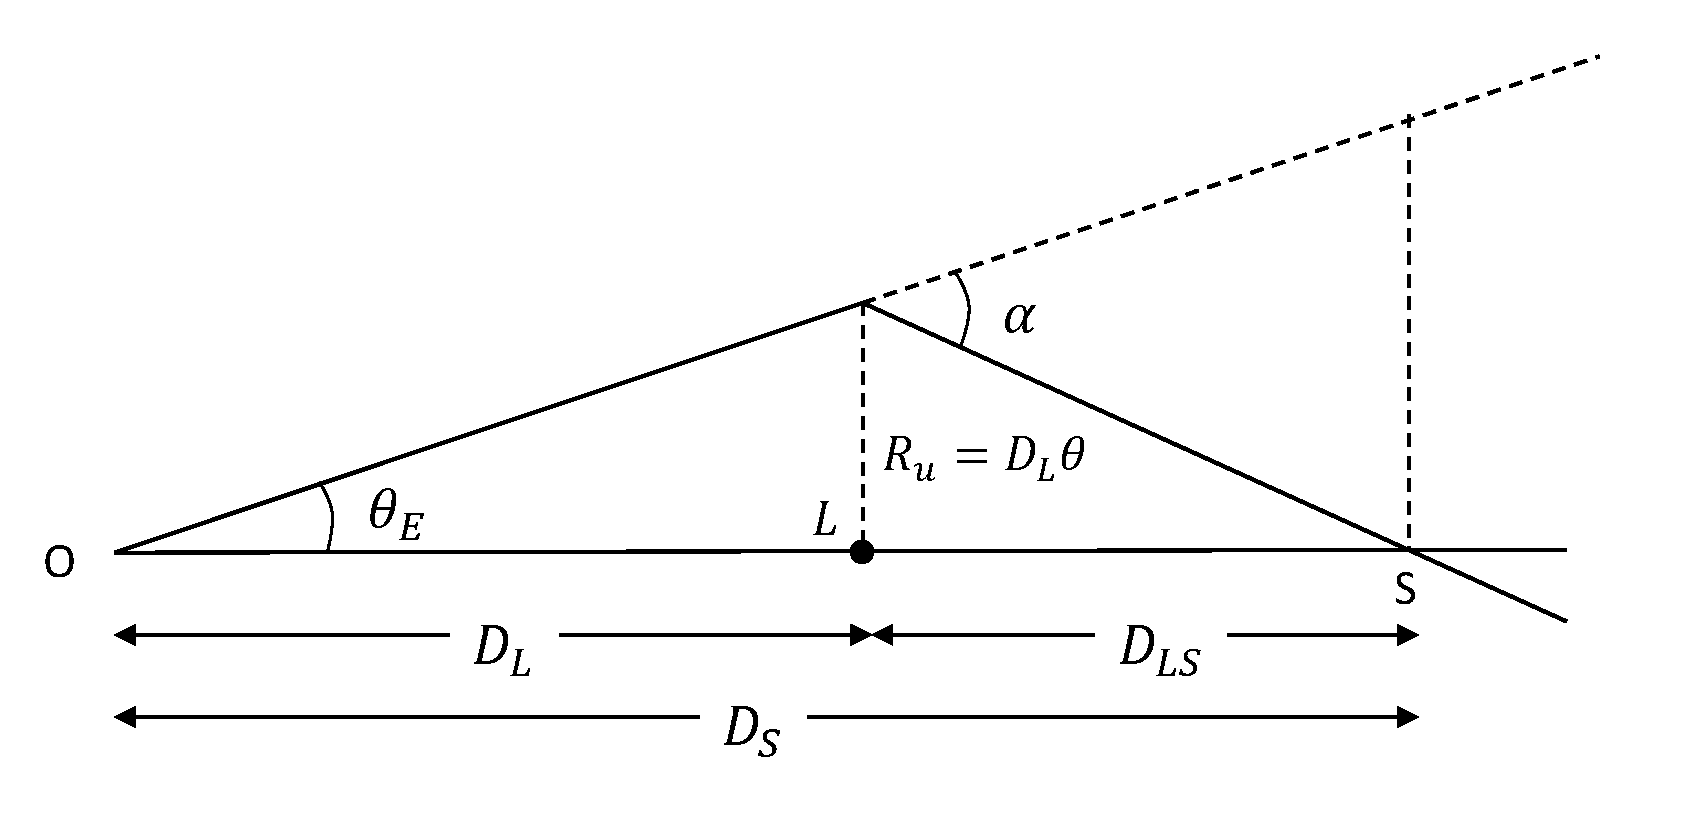
\includegraphics[height=0.4\linewidth]{images/lensing_cropped.pdf}
  \caption{Diagram of gravitational lensing, where the lens, observer, and source are collinear.}
  \label{fig:lensing}
\end{figure}

We consider a simple picture where the observer, lens, and source are aligned, as shown in \autoref{fig:lensing}. Bending is assumed to happen at a single point above the lens, since the distance from the observer to the lens and source is assumed to be much larger than the distance of closest approach between the light ray and the lens. From this diagram we can easily, with some trigonometry, obtain the lens equation \citep{schneider1992gravitationallenses}

\begin{equation}
  D_S \theta_E = D_{LS} \alpha
  \label{eq:lens-eqn}
\end{equation}
where $\alpha$ is the bending angle as previously derived, $D_S$ is the angular diameter distance from observer to source, $D_{LS}$ is the angular diameter distance from lens to source, and $\theta_E$ is known as the Einstein angle. $R_u$ can also be expressed in terms of the observable quantities $R_u = D_L \theta_E$, where $D_L$ is the angular diameter distance from observer to the lens.  

With this in mind, we can begin looking at the Swiss-cheese model, and look to apply this formalism in such a universe. 
  %!TEX root = ../thesis.tex
\chapter{Description of the Swiss-cheese model}
\label{chapter:swiss-cheese}

\section{Spacetime patches}

Swiss-cheese (SC) models were first introduced by \citet{einstein1945influence} to investigate the gravitational field of a mass well described by the Schwarzschild metric but embedded in a non-Minkowski background spacetime. Such a model is contructed by removing a comoving sphere from the homogeneous background and replacing it with an inhomogeneous mass distribution (see \autoref{fig:swiss-cheese}). In this case, we use a mass distribution that is vacuum everywhere except for a point mass at the centre. In principle, since the sphere is comoving, multiple spheres can be inserted in the cheese as long as they are initially non-overlapping. In our model, only one hole is needed to model the lens. This stitching of two metrics on the cheese-hole boundary is of course not arbitrary, and matching conditions will impose restriction on the parameters of the two metrics. This will be discussed in detail in the following sections. 

\begin{figure}
  \centering
  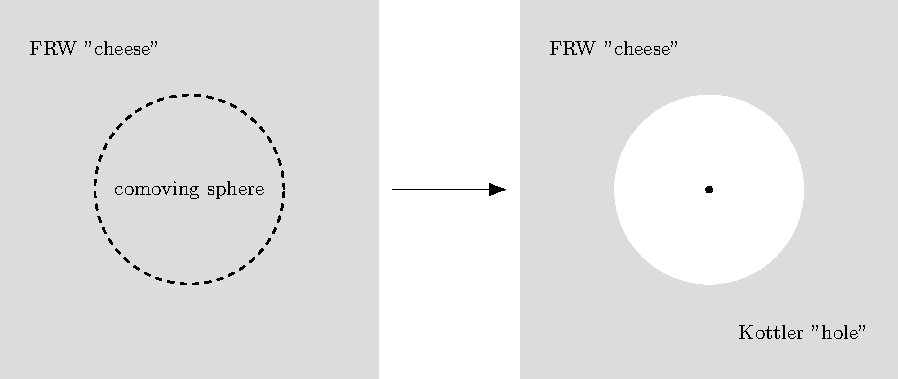
\includegraphics[height=0.3\linewidth]{images/swiss-cheese.pdf}
  \caption{Construction of a Swiss-cheese model}
  \label{fig:swiss-cheese}
\end{figure}

There are several reasons why this model was chosen. First, this is an exact solution of Einstein's equations which preserves the global dynamics, and hence it will allow us to properly investigate the higher order corrections that have been oft-debated in literature. Secondly, by putting observers in the homogeneously expanding "cheese", it accounts for observers moving with the Hubble flow, which is a common objection to Rindler and Ishak's use of a static metric \citep{park2008rigorous,khriplovich2008does,simpson2010lensing,butcher2016no}. Lastly, this model also takes the finite range of the mass into account by confining the influence of the central mass to the size of the hole. 

Light propagation in SC models has been extensively studied \citep{szybka2011light,vanderveld2008luminosity,fleury2014swiss}, but not particularly so in the subject of the $\Lambda$ dependence on gravitational lensing. Some of the areas that Swiss-cheese models have been commonly used include investigating the effect of local inhomogeneities on luminosity-redshift relations \citep{kantowski1969corrections,fleury2013interpretation} and studying fluctuations in redshift and distance of the cosmic microwave background \citep{bolejko2009szekeres,valkenburg2009swiss,bolejko2011effect}. 

A significant difference between the Swiss-cheese model and what is used in conventional gravitational lensing, as described in the previous section, is that in the Swiss-cheese, the bending happens only inside the hole, whereas in conventional lensing, the mass is superimposed on the FRW background and has infinite range. In the Swiss-cheese model, due to the boundary conditions, all bending is truncated once the light ray leaves the hole, and outside the hole the light ray travels as if the hole does not exist. Therefore even in the $\Lambda = 0$ case, we would expect a slightly smaller bending angle in the Swiss-cheese than predicted in conventional lensing, even though this difference is small. 

\citet{kantowski2010gravitational} did analytical calculations in estimating the bending angle in the Swiss-cheese model in flat space (see Eq. 32 of \citet{kantowski2010gravitational}). This prediction, together with the conventional lensing prediction (\autoref{eq:series-expansion-R}) and the Rindler and Ishak prediction (\autoref{eq:rindler-ishak-alpha}), are the theoretical models that we will be comparing our numerical results against. 

% In the Swiss-cheese model, in principle multiple holes can be inserted into the cheese. In this project, we use a single hole for the lens. 

\subsection{Friedmann-Robertson-Walker geometry}

Outside the hole, geometry is described by the Friedmann-Robertson-Walker (FRW) metric, the simplest homogeneous and isotropic model of the universe. Its line element, in spherical polar coordinates, is given by \citep{wald2010general}

\begin{equation}
  ds^2 = -dt^2 + a(t)^2 \left ( \frac{dr^2}{1-kr^2} + r^2 d \Omega^2 \right )
  \label{eq:frw-metric}
\end{equation}
where $d \Omega^2 = d\theta^2 + \sin^2\theta d\phi^2$ is the metric on a 2-sphere, $a(t)$ is the varying scale factor of the universe, and $k$ represents the curvature of space. This is the line element for a homogeneous and expanding universe with general spatial curvature. There are 3 possibilities for the value of $k$, each implying a different geometry of the universe:

\begin{itemize}
  \item $k = 0$: The universe is flat and Euclidean.
  \item $k > 0$: The universe has positive spatial curvature and is closed
  \item $k < 0$: The universe has negative spatial curvature and is open. 
\end{itemize}

The scale factor $a$ parametrises the relative expansion of the universe, such that the relationship between physical distance and comoving distance between two points at a certain cosmic time $t$ is given as

\begin{equation}
  d_{\text{physical}} = a(t) d_{\text{comoving}}.
  \label{eq:comoving-physical-distance}
\end{equation}

The scale factor also satisfies the Friedmann equation

\begin{equation}
  H^2 \equiv \left ( \frac{1}{a}\frac{da}{dt} \right )^2 = \frac{8\pi G \rho}{3} + \frac{\Lambda}{3} - \frac{k}{a^2}
  \label{eq:friedmann-equation}
\end{equation}
where $\rho$ is the energy density of a pressureless fluid and $H$ is the Hubble parameter. 

It is common to introduce the cosmological parameters, where a subscript 0 refers to quantities evaluated today: 

\begin{equation}
  \Omega_m = \frac{8\pi G \rho_0}{3H_0^2}, \,\, \Omega_{\Lambda} = \frac{\Lambda}{3H_0^2}, \,\, \Omega_k = - \frac{k}{a_0^2 H_0^2}
  \label{eq:cosmo-params}
\end{equation}
and rewrite the Friedmann equation as

\begin{equation}
  H^2 = H_0^2 \left [ \Omega_m \left ( \frac{a_0}{a}\right )^3 + \Omega_k \left ( \frac{a_0}{a}\right )^2 + \Omega_{\Lambda} \right ]
  \label{eq:friedmann-eqn-version2}
\end{equation}
where the $\Omega$ terms are commonly known as density parameters, evaluated at the present day. In the absence of radiation, they obey the relation

\begin{equation}
  \Omega_m + \Omega_{\Lambda} + \Omega_k = 1.
  \label{eq:density-parameters-1}   
\end{equation} 

In a flat universe, space is Euclidean and $\Omega_k = 0$. 

% Subsequently in this report instead of working directly with $\Lambda$ I will work with $\Omega_{\Lambda}$ instead. 

\subsection{Kottler geometry}

In this project we use a Kottler condensation in the Swiss-cheese for the central lensing mass. This is described by a Kottler metric \citep{kottler1918physikalischen}, which is the extension of the famous Schwarzschild metric to include a cosmological constant, given by

\begin{equation}
  ds^2 = -f(R)dT^2 + \frac{dR^2}{f(R)} + R^2 d \Omega^2
  \label{eq:kottler-metric}
\end{equation}
with
\begin{equation}
  f(R) = 1-\frac{2M}{R} - \frac{\Lambda R^2}{3},
  \label{eq:kottler-metric-f}
\end{equation}
where M is the mass of the central object. Unlike the FRW, this metric describes a static spacetime. 

\section{Matching conditions}

Two geometries can be matched across the boundary to form a well defined spacetime if and only if they satisfy the Darmois-Israel junction conditions \citep{darmois1927equations,israel1966singular}. These conditions dictate that the first and second fundamental forms of the two metrics must match on the matching hypersurface $\Sigma$, that is, both metrics must induce 
\begin{inparaenum}[(i)]
  \item the same metric, and 
  \item the same extrinsic curvature.
\end{inparaenum}

\subsection{Continuity of the induced metric}

We match the FRW and Kottler metrics on a surface of a comoving 2-sphere, $\Sigma$, which is defined by $r = r_h = \text{constant}$ in FRW coordinates and $R = R_h(T)$ in Kottler coordinates.

The induced metric is the quantity 

\begin{equation}
  h_{ab} = g_{\alpha \beta} j^{\alpha}_{a} j^{\beta}_{b}
  \label{eq:induced-metric-defn}
\end{equation}
where $j^{\alpha}_{a}$ is defined as

\begin{equation}
  j^{\alpha}_{a} = \frac{\partial \bar{X}^{\alpha}}{\partial \sigma^a}.
  \label{eq:j-defn}
\end{equation}
Here we have introduced $X^{\alpha}$ to represents coordinates of the original metric. We define $\sigma^a$ to be natural intrinsic coordinates for $\Sigma$, and $\bar{X}^{\alpha}(\sigma^a)$ is the parametric equation of the hypersurface. 

More concretely, using the coordinates defined previously in \autoref{eq:frw-metric}, these quantities are, for the FRW, 

\begin{subequations}
  \begin{align}
    X^{\alpha} &= \{ t, r, \theta, \phi \} \\
    \sigma^a &= \{ t, \theta, \phi \} \\
    \bar{X}^{\alpha}(\sigma^a) &= \{ t, r_h, \theta, \phi\}.
  \end{align}
\end{subequations}

Similarly, in the Kottler region, we have 

\begin{subequations}
  \begin{align}
    X^{\alpha} &= \{ T, R, \theta, \phi \} \\
    \sigma^a &= \{ T, \theta, \phi \} \\
    \bar{X}^{\alpha}(\sigma^a) &= \{ T, R_h(T), \theta, \phi\}.
  \end{align}
\end{subequations}

Using these definitions, the 3-metric induced by the FRW geometry on $\Sigma$ is

\begin{equation}
  ds^2_{\Sigma} = -dt^2 + a^2(t)r^2 d \Omega^2,
  \label{eq:frw-induced-metric}
\end{equation}
while the induced metric on the Kottler metric is
\begin{equation}
  ds_{\Sigma}^2 = -\kappa^2(T)dT^2 + R_h^2(T) d \Omega^2,
  \label{eq:kottler-induced-metric}
\end{equation}
where
\begin{equation}
  \kappa \equiv \sqrt{\frac{f^2[R_h(T)] - \left(\frac{dR_h(T)}{dT}\right)^2}{f[R_h(T)]}}.
  \label{eq:kottler-kappa}
\end{equation}

Equating the components of \autoref{eq:frw-induced-metric} and \autoref{eq:kottler-induced-metric}, we obtain the following:

\begin{equation}
  R_h(T) = a(t)r
  \label{eq:r-to-ar},
\end{equation}

\begin{equation}
  \frac{dt}{dT} = \kappa(T).
  \label{eq:dt-dT}
\end{equation}

% \begin{subequations}
%   \begin{align}
%     R_h(T) = a(t)r \\
%     \frac{dt}{dT} = \kappa(T).
%   \end{align}
% \end{subequations}

These two relationships relate the radial and time coordinates of the two metrics respectively. 

\subsection{Continuity of the extrinsic curvature}

The second condition equates extrinsic curvature of the two geometries. By definition, the extrinsic curvature $K_{ab}$ of a hypersurface is given by

\begin{equation}
  K_{ab} = n_{\alpha;\beta} j^{\alpha}_{a} j^{\beta}_{a}
  \label{eq:extrinsic-curvature-defn}
\end{equation}
where $n_{\mu}$ is the unit vector normal to $\Sigma$, $j$ is as defined previously in \autoref{eq:j-defn}, and the semicolon notation `;' denotes a covariant derivative, for example, $n_{\alpha;\beta} = \nabla_{\beta}\, n_{\alpha}$. For any vector $V^{\nu}$, the covariant derivative is defined as

\begin{equation}
  \nabla_{\mu}V^{\nu} = \partial_{\mu}V^{\nu} + \Gamma^{\nu}_{\mu \rho} V^{\rho}.
  \label{eq:covariant-derivative-defn}
\end{equation}

For a hypersurface defined by a function $q = 0$, the unit vector normal to it is

\begin{equation}
  n_{\mu} = \frac{q_{,\mu}}{\sqrt{g^{\alpha \beta} q_{,\alpha} q_{,\beta}}}.
  \label{eq:unit-normal-vector}
\end{equation}

In our case $q = r-r_h$ in FRW coordinates and $q = R - R_h(T)$ in Kottler coordinates. For example, the unit vector in the FRW region is trivial to calculate, and we get $n_{\mu}^{\text{(FRW)}} = \delta^r_{\mu}/a$. Applying this formula, the extrinsic curvature induced by the FRW geometry is

\begin{equation}
  K_{ab} dx^a dx^b = \frac{a(t)r}{\sqrt{1-kr^2}} d \Omega^2
  \label{eq:extrinsic-curvature-frw}
\end{equation}
while the extrinsic curvature induced by the Kottler geometry is
\begin{equation}
  K_{ab} dx^a dx^b = \frac{1}{\kappa} \left [ \frac{d^2R_h}{dT^2} + \frac{f^{\prime}}{2f}\left (f^2 - 3 \left (\frac{dR_h}{dT}\right )^2 \right) \right] dT^2 + \frac{R_h f}{\kappa} d \Omega^2
  \label{eq:extrinsic-curvature-kottler}
\end{equation}
where $f^{\prime} = \partial f / \partial R$, and all quantities are evaluated at $R = R_h(T)$.

Equating the components of \autoref{eq:extrinsic-curvature-frw} and \autoref{eq:extrinsic-curvature-kottler}, we obtain

\begin{equation}
  \frac{R_h f}{\kappa} = \frac{a(t)r}{\sqrt{1-kr^2}}
  \label{eq:kappa-to-fprime}
\end{equation}
and
\begin{equation}
  \frac{d^2R_h}{dT^2} + \frac{f^{\prime}}{2f}\left [f^2 - 3 \left (\frac{dR_h}{dT}\right )^2 \right ] = 0.
\end{equation}
The second equation is provided for completeness although it is not needed for subsequent derivations. 

\subsection{Consequences on properties of the hole}

Combining \autoref{eq:kappa-to-fprime} with \autoref{eq:kottler-kappa}, we can eliminate $\kappa$. We can also replace $dR_h/dT$ using the relation obtained in \autoref{eq:r-to-ar}, since

\begin{equation}
  \frac{dR_h}{dT} = \frac{d(ar)}{dT} = \frac{da}{dt}\frac{dt}{dT}r.
\end{equation}
where $da/dt$ is given by the Friedmann equation \ref{eq:friedmann-equation}. Following through with the algebra, we arrive at the somewhat intuitive result that both regions must have the same cosmological constant $\Lambda$ and that the Kottler hole has to be mass compensating, meaning the enclosed mass $M$ has to equal the mass excised from the FRW background:

\begin{equation}
  M = \frac{4\pi}{3} \rho a^3 r_h^3. 
  \label{eq:junction-conditions-mass-volume}
\end{equation}

From the junction conditions the rate of expansion of the hole in static coordinates can also be obtained. By combining \autoref{eq:kottler-kappa} and \autoref{eq:kappa-to-fprime}, we get an expression for $dR_h/dT$

\begin{equation}
  \frac{dR_h}{dT} = f(R_h) \sqrt{1- \frac{f(R_h)}{1-k r_h^2}}.
  \label{eq:hole-expansion-in-kottler-dR-dT}
\end{equation}

The last thing we need from the boundary conditions is to relate the tangent vectors between the two metrics. The continuity of the metric, imposed by the first junction condition, implies that the connection does not diverge across the boundary. Therefore, light is not deflected as it crosses the boundary and we just need to convert the components of the tangent vector between the two coordinate systems. To obtain $\dot{R}$ in terms of FRW tangent vectors $\dot{r}$ and $\dot{t}$, we differentiate \autoref{eq:r-to-ar} and substitute $da/dt$ with the Friedmann equation \autoref{eq:friedmann-equation}. Keeping in mind the boundary conditions, we get an expression for $\dot{R}$. The angular coordinates and angular tangent vectors are unchanged when moving from the Kottler to FRW coordinates, and vice versa. With $\dot{R}$ and $\dot{\phi}$, $\dot{T}$ then can be easily obtained from the null condition \autoref{eq:null-condition}. The result is

\begin{subequations}
  \begin{align}
    \dot{T} &= \frac{\dot{t}}{f}\sqrt{1-kr^2} + \frac{a\dot{r}}{f\sqrt{1-kr^2}} \sqrt{\frac{2M}{ar} - kr^2 + \frac{\Lambda}{3}a^2 r^2} \\
    \dot{R} &= \dot{t}\sqrt{\frac{2M}{ar} - kr^2 + \frac{\Lambda}{3}a^2 r^2} + a\dot{r}\\
    \dot{\phi} &= \dot{\phi}\\
    \dot{\theta} &= \dot{\theta}
  \end{align}
  \label{eq:kottler-to-frw-transform-jacobian}%
\end{subequations}
where for completeness I have also given the trivial relations between the angular tangent vectors. The quantities above are all evaluated at the boundary of the hole. This result is given for flat space in \citet{schucker2009strong} and \citet{fleury2013interpretation}, but here it has been extended to allow for arbitrary spatial curvature. The reverse transformation is easily obtained by inverting the Jacobian from above. 

In summary, given a FRW spacetime with pressureless matter and a cosmological constant $\Lambda$, a spherical hole, whose geometry is described by the Kottler metric, can be constructed which contains a constant mass $M = 4\pi \rho a^3 r_h^3/3$ at its centre. The geometry resulting from combining the two metrics at the boundary is an exact solution of the Einstein field equations. Applying the boundary conditions, we can obtain all the necessary transformations needed for continuation of light propagation at the boundary. 

\section{Light propagation}

We propagate a light ray backwards from observer to source by solving the geodesic equation (\autoref{eq:geodesic-eqn}). In reality, the light ray travels from source to observer, but our calculations proceed in the opposite direction since we want to take the current observer position and observation event as the initial condition. The observer is placed in the FRW region, where we start propagating the light ray. The mass of the lensing object is fixed and consequently so is the size of the hole. The light ray is started off with an Einstein angle $\theta_{E}$, travels through the FRW region, encounters the Kottler hole which deflects its trajectory, and returns to the FRW region again (see \autoref{fig:swiss-cheese-ray}. In the Swiss-cheese model, all the bending occurs only in the Kottler hole and is truncated once light leaves the hole. 

\begin{figure}
  \centering
  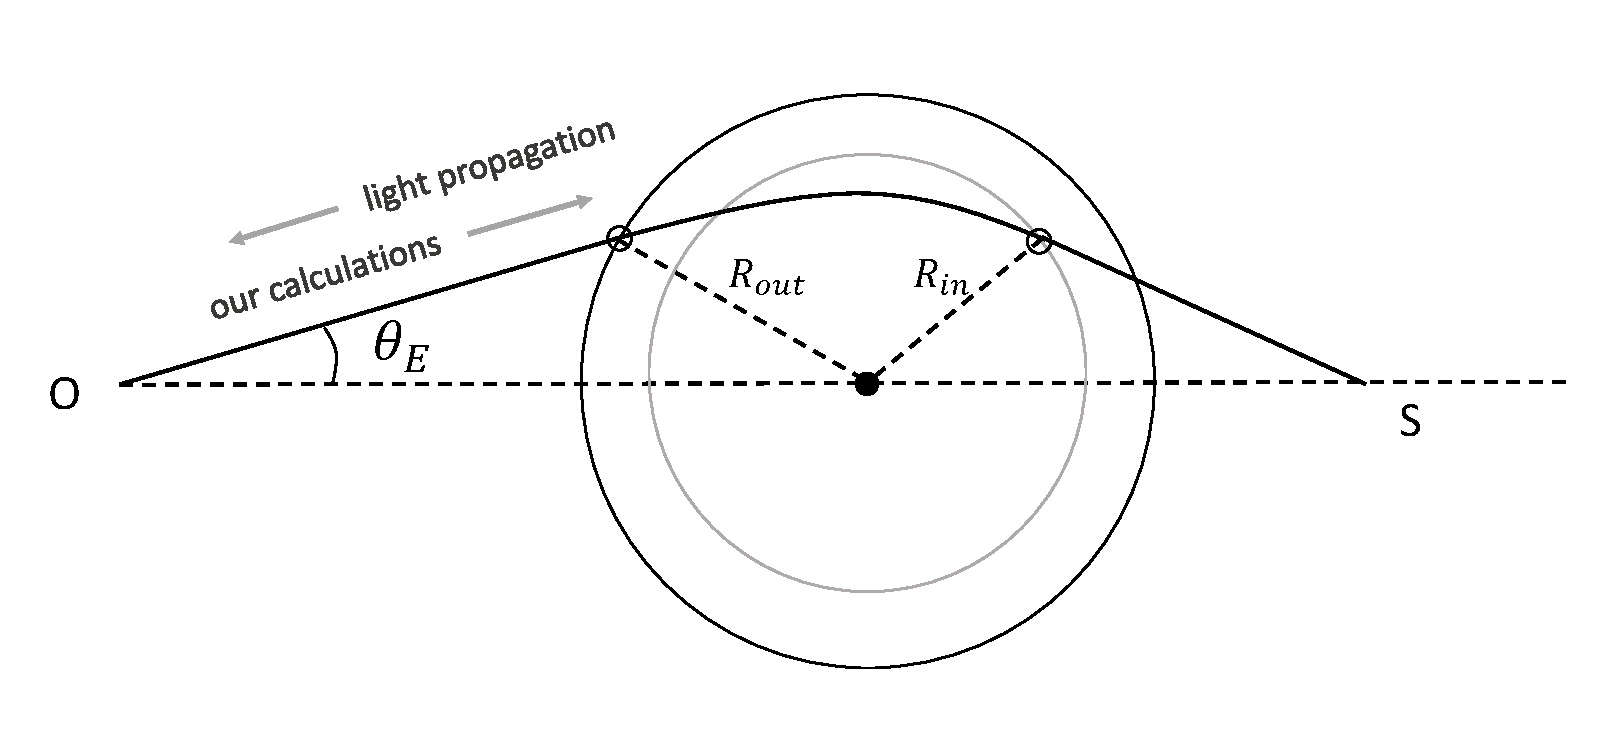
\includegraphics[height=0.4\linewidth]{images/swiss-cheese-ray2-cropped.pdf}
  \caption{A diagram of how a light ray propagates through the Swiss-cheese. Our calculations are done in the opposite direction of propagation. Due to the expansion of the universe, the physical size of the hole will be larger when the light exits the hole compared to when it entered.}
  \label{fig:swiss-cheese-ray}
\end{figure}

We begin by fixing the lens redshift, since it is the redshift that is directly observable and not the radial coordinate $r$. From the lens redshift, we can then calculate the radial coordinate and angular diameter distance to the lens. 

In the FRW, assuming $a_0 = 1$, we can calculate the angular diameter distance $D_L$ for a given lens redshift $z_L$ as \citep{hogg1999distance}

\begin{equation}
  D_L = D_A(z_L) = \frac{1}{1+z_L} S_k\left ( \frac{1}{H_0}\int_0^{z_L} \frac{dz}{\sqrt{\Omega_m(1+z)^3 + \Omega_k (1+z)^2 + \Omega_{\Lambda}}}  \right )
  \label{eq:angular-diameter-distance-redshit-z}
\end{equation}
where we define the function $S_k(x)$

\begin{equation}
  S_k(x) = 
  \begin{cases}
    \mathopen| k \mathclose|^{-1/2} \sin(\sqrt{\mathopen| k \mathclose|}x) & k > 0\\
    x & k = 0\\
    \mathopen| k \mathclose|^{-1/2} \sinh(\sqrt{\mathopen| k \mathclose|}x) & k < 0
  \end{cases}
  \label{eq:sk}
\end{equation}
and its inverse function

\begin{equation}
  S_k^{-1}(x) = 
  \begin{cases}
    \mathopen| k \mathclose|^{-1/2} \sin^{-1}(\sqrt{\mathopen| k \mathclose|}x) & k > 0\\
    x & k = 0 \\
    \mathopen| k \mathclose|^{-1/2} \sinh^{-1}(\sqrt{\mathopen| k \mathclose|}x) & k < 0
  \end{cases}
  \label{eq:sk-inverse}
\end{equation}

In terms of the angular diameter distance, the radial coordinate is given by 

\begin{equation}
  r_L = (1+z_L)D_L.
\end{equation}

Therefore, as we vary $\Lambda$, $r_L$ is expected to change since we fix $z_L$. We then place the lens at the origin and observer at a radial coordinate of $r = r_L$ and $\phi = \pi$. 

Numerical integration is done with the \texttt{scipy.integrate.solve\_ivp} function in Python \citep{jones2014scipy}, which uses an explict Runge-Kutte method of order $5$ \citep{dormand1980family}. The solver uses an adaptive step size, and the intersection between the light ray and the point of entry and exit of the hole are found with the classic Brent's method \citep{brent2013algorithms}, a root-finding algorithm. 

\subsection{FRW region}

The light ray begins from the observer in the FRW region. The starting tangent angle $\theta_E$ is fixed, and the initial tangent vectors are set such that $\theta_E = \tan^{-1}(\sqrt{1-kr^2}r\dot{\phi}/\dot{r})$. We place the lens at the origin and take the observer to be at an azimuthal angle of $\phi = \pi$. 

Null geodesics govern the trajectory of the light ray. Without loss of generality, we can take $\theta = \pi/2$ to simplify the geodesic equations. Due to spherical symmetry, the FRW has a conserved quantity $L = a^2 r^2 \dot{\phi}$ that corresponds to the angular momentum of the photon. In terms of the conserved quantity, the null geodesic equations are

\begin{subequations}
  \begin{align}
    \dot{t} &= -\sqrt{\frac{a^2\dot{r}^2}{1-kr^2} + a^2r^2 \dot{\phi}}\\
    \ddot{r}  &= (1-kr^2)r\dot{\phi}^2 - \frac{kr\dot{r}^2}{1-kr^2} - \frac{2a_{,t}}{a}\dot{r}\dot{t}\\
    \dot{\phi} &= \frac{L}{a^2 r^2}
  \end{align}
  \label{eq:frw-null-geodesics}%
\end{subequations}
which, when combined with the Friedmann equation (\autoref{eq:friedmann-eqn-version2}), fully determine the light's path. The negative sign on $\dot{t}$ is due to the fact that we are propagating the light backwards in time. We can then solve these differential equations numerically and stop the integration once the light ray reaches the boundary of the hole, which is defined by $r_h = \text{constant}$. We call this intersection event $\mathcal{E}_{\text{out}}$, since this is where the light, traveling from the source to observer in the opposite direction of our numerical calculations, \emph{leaves} the hole. 

In the particular case of Euclidean geometry ($k = 0$), the coordinates of the event $\mathcal{E}_{\text{out}}$ can be calculated analytically. To do this, we first rewrite the flat metric in terms of the conformal time $\eta$, defined by $d\eta = dt/a(t)$, as

\begin{equation}
  ds^2 = a^2(\eta) \left ( -d \eta^2 + dr^2 + r^2 d \Omega^2 \right ).
  \label{eq:frw-metric-conformal-time}
\end{equation}

We can then write down the following system of equations in Cartesian coordinates $x^i_{\text{out}}$, in terms of the hole radius $r_h$ and Cartesian position of the observer $x^i_0$:

\begin{subequations}
  \begin{align}
  \delta_{ij} (x^i_{\text{out}} - x^i_h)(x^j_{\text{out}} - x^j_h) = r_h^2\\
  x^i_{\text{out}} = x^i_0 + (\eta_0 - \eta_{\text{out}})d^i    
  \end{align}
  \label{eq:flat-cartesian-frw}%
\end{subequations}
where $d^i$ is the unit vector representing direction of travel. For a given Einstein angle $\theta_E$, in Cartesian coordinates we have 

\begin{align}
    d &= \frac{1}{\sqrt{(\dot{r}\cos\phi - r\sin\phi\dot{\phi})^2 + (\dot{r}\sin\phi + r\cos\phi\dot{\phi})^2}}
          \begin{pmatrix}
           \dot{r}\cos\phi - r\sin\phi\dot{\phi} \\
           \dot{r}\sin\phi + r\cos\phi\dot{\phi} \\
         \end{pmatrix}
\end{align}

The final thing we need is to recover the scale factor from the conformal time. From \autoref{eq:flat-cartesian-frw}, we can obtain the value of $\eta_{\text{out}}$, since we can arbitrarily set $\eta_0 = 0$. We take $a_0 = 1$ at the observer, so the conformal time $\eta$ is related to $a$ by

\begin{equation}
  \eta_{\text{out}} = \frac{1}{H_0} \int_1^{a_{\text{out}}} \frac{1}{a^2 \sqrt{\Omega_m/a^3 + \Omega_{\Lambda}}}.
  \label{eq:conformal-time-eta-to-a-integral}
\end{equation}
where $H_0$ is the current value of the Hubble parmeter. Since $\eta$ increases monotonically with $a$, we did a simple binary search to find the value of $a_{\text{out}}$ that produced $\eta_{\text{out}}$ to the required level of accuracy. 

The above calculation only applies for flat space, and in arbitrarily curved space, we do the full numerical integration to obtain the conditions at $\mathcal{E}_{\text{out}}$.

\subsection{Conversion from FRW region to Kottler region at $\mathcal{E}_{\text{out}}$}
\label{subsec:frw-to-kottler}

From the FRW coordinates and tangent vectors, we can first obtain the starting coordinate $R_{\text{out}}$ from \autoref{eq:r-to-ar}. The angular coordinates remain the same in both coordinate systems. We are free to set $T_{\text{out}} = 0$ since we are not concerned with the amount of time taken by the light, only the trajectory. 

The initial tangent vectors to start off the Kottler integration can be obtained from the Jacobian derived in the previous section (\autoref{eq:kottler-to-frw-transform-jacobian}).

\subsection{Kottler region}

Inside the hole, the staticity and spherical symmetry of the Kottler metric imply the existence of two conserved quantities, $E = f(R) \dot{t}$ and $L = R^2 \dot{\phi}$, which correspond to the energy and angular momentum of the photon respectively. The null condition, after rearranging to make $\dot{R}$ the subject, reads

\begin{equation}
  \dot{R} = \pm \sqrt{E^2 - \frac{L^2}{R^2} \left ( 1 - \frac{2M}{R} - \frac{\Lambda R^2}{3}\right )}.
  \label{eq:kottler-null-condition}
\end{equation}
The $\pm$ before square root on the right hand side is troublesome for numerical computations because it would become necessary to determine a point to switch signs for $\dot{R}$. To circumvent that, we can differentiate the equation obtained from the null condition to get a second order differential equation in $R$. Combining that with the conserved quantities, we have the following equations which fully determine the light trajectory in Kottler space:

\begin{subequations}
  \begin{align}
    \dot{T} &= \frac{E}{f(R)}\\
    \ddot{R}  &= \frac{L^2 (R-3M)}{R^4}\\
    \dot{\phi} &= \frac{L}{R^2}.
  \end{align}
  \label{eq:kottler-null-geodesics}%
\end{subequations}
Note that the second order differential equation in $R$ now has no dependence on $\Lambda$, which is the aforementioned conventional argument pioneered by \citet{islam1983cosmological} for why $\Lambda$ does not directly contribute to lensing. 

At the same time that the light ray is moving through the Kottler hole, the hole boundary is also changing in the static coordinates, with an expansion rate governed by \autoref{eq:hole-expansion-in-kottler-dR-dT}. This equation needs to be integrated simulataneously with the null geodesic equations in order to find the point that the light ray intersects with the hole again. We call this event $\mathcal{E}_{\text{in}}$, again to emphasize the fact that this is where light enters the hole, although the propagation is done in the opposite direction. 

\subsection{Conversion from Kottler region to FRW region at $\mathcal{E}_{\text{in}}$}

Conversion from the Kottler to FRW region is simply the reverse of the transformations stated in \autoref{subsec:frw-to-kottler}. We set $t_{\text{in}} = 0$ since we are not concerned with the path time. 

\subsection{Back in the FRW region}

Once we get back to the FRW region, we continue using FRW null geodesics (\autoref{eq:frw-null-geodesics}) to propagate the light and stop once we reach the axis. The coordinate at which it crosses the axis is then recorded. 

In flat space, numerical integration here is no longer necessary, since there will be no more bending in this region. Thus the intersection of the light path with the axis can be calculated from the tangent vector directly once light exits the Kottler hole. 

\subsection{Converting raw radial coordinates to angular diameter distances}

Our aim is to compare our results against the cosmological lens equation (\autoref{eq:lens-eqn}), using strictly observable quantities. Gravitational lensing analysis is usually done with us (the observer) at the origin, but in our model we have placed the lens at the origin instead out of convenience. Therefore we take extra care when converting from raw radial coordinates back into observable angular distances. By an extension of the redshift formula (\autoref{eq:angular-diameter-distance-redshit-z}), we can get the angular diameter distance between two arbitrary points given their respective radial coordinates \citep{peacock1999cosmological}

\begin{equation}
  D_{AB} = \frac{a_0  S_k(S_k^{-1}(r_B) - S_k^{-1}(r_A))}{1+z_B}
\end{equation}

Applying this formula and remembering that we place the observer at $(r, \phi) = (r_L, \pi)$, we can use our final numerical coordinate at $(r, \phi) = (r_{LS}, 0)$ to get $D_S$ and $D_{LS}$:

\begin{subequations}
  \begin{gather}
    D_{S} = \frac{S_k(S_k^{-1}(r_{LS}) + S_k^{-1}(r_L))}{1+z_S}\\
    D_{LS} = \frac{r_{LS}}{1+z_S}
  \end{gather}
\end{subequations}

With this, we now have all the formulation needed to carry out the numerical integration and also to translate the numerical results into observable quantities. 

We also extend this model beyond a Kottler hole to a general static mass distribution, by replacing the Kottler metric by a LTB metric with pressure and deriving the null geodesics again in this spacetime. The quantities and results for the LTB metric are presented in \autoref{appendix:ltb}.
  %!TEX root = ../thesis.tex
\chapter{Results and discussion}
\label{chapter:results}

A graph of results when we keep the lensing mass $M$ constant and vary $\Omega_{\Lambda}$ can be seen in [fig??]. On the $y$-axis, we have plotted the the deviation of $\alpha$ as a fraction of the standard FRW lensing case (given by [eq??]), in order to put them on the same scale. [State te mass and zlens parameters] 

By varying the integration step size, we are able to estimate numerical errors on the integration. For a certain step size, we group the results obtained from the vicinity of step sizes together and find the variance in bending angles in that range. Fig [??] shows how the $\alpha$ obtained varies with step size. As is expected, the precision increases as we reduce the step size. 

Our results seem to follow the trend of Kantowski's predictions most closely, with a gap that reduces towards higher $\Lambda$. A possible explanation of this gap can be found by examining the neglected higher order term in Kantowski's predicted bending angle [eq??]. When $\Lambda = 0$, the ratio of this term to the leading order $(4M/r_0^2) \cos^3 \tilde{\phi_1}$ term is of the same order of magnitude as the fractional deviation of our numerical results from Kantowski's predictions. As is expected, this ratio decreases as $\Lambda$ when mass is kept constant, as can be seen from [fig??]. 

From the graph, we can see that even for the $\Lambda = 0$ case there is an offset between the numerical Swiss-Cheese result and the FRW prediction. Qualitatively, this is due to the fact that conventional lensing analyis assumes a mass superimposed on the homogeneous background, and this mass has infinite range. However, in the Swiss-Cheese model, the influence of the mass is limited, and bending stops once it leaves the Kottler hole. This is the main effect that Kantowski quantified in his paper \citet{kantowski2010gravitational}. This then begs the question of which model is a more accurate description of our physical universe, but this is not our primary concern. We are concerned about whether $\Lambda$ has an influence on this effect. 

There are a few different factors at play here. In discussing the results of this numerical integration, let us take a step back to look at the specific parts of ray-tracing that have a $\Lambda$-dependence. These are:
\begin{enumerate}
  \item The size of the hole. This is governed by \autoref{eq:junction-conditions-mass-volume}. In flat space, increasing $\Omega_{\Lambda}$ implies decreasing $\Omega_{\Lambda}$, which corresponds to the matter density of the universe. If we are to keep the mass constant, the hole size would have to increase as we increase $\Omega_{\Lambda}$. 
  \item The rate of expansion of the hole in static Kottler coordinates, given by [ref??].  
  \item The Jacobian at the boundary, given by [??]
\end{enumerate}

The first effect does not seem to be a truly direct $\Lambda$ effect, merely a side effect that in a flat universe, changing $\Omega_{\Lambda}$ must imply a change in matter density, but ultimately, it is the size of the hole that is the true determining factor. 
  %!TEX root = ../thesis.tex
\chapter{Conclusion}
\label{chapter:conclusion}

In this work, we examined gravitational lensing in a Swiss-Cheese model that has an embedded Kottler hole. We numerically integrated null geodesics in such a universe piecewise and calculated lensing observables from the numerical results. These results were compared with predictions by Rindler \& Ishak and Kantowski. Our results appear to agree most with Kantowski's predictions, with a small varying gap that can be explained by the presence of higher order terms not considered in Kantowski's results. 

However, it is difficult to isolate the effect of $\Lambda$, since a change in $\Lambda$ \emph{must} involve a change in either $\Omega_m$ or $\Omega_k$, and it is not clear at the outset which quantity should be kept constant as we turn up $\Lambda$. We looked into case where spatial curvature compensates for the change in $\Lambda$, but from our results it appears that $\Omega_k$ has a much larger effect than $\Lambda$ on lensing observables in the Swiss-Cheese model, so we focused on looking at results from a spatially flat Universe. 

We kept the hole size constant while varying $\Lambda$ to eliminate any effect coming from the size of the hole that might be considered a $\Lambda$ effect. Even so, $\Lambda$ appears to have an effect on the lensing observables, although this effect is small---smaller than the size of the second order term in $M/R_u$, which is routinely neglected. 

\section{Future work}

Our work is focused solely on the collinear case, in which the source, lens and observer are aligned, but it is straightforward to generalize beyond this restriction. 

The case with curvature somewhat glossed over, since curvature appeared to have a much larger influence than $\Lambda$, and most work done on embedded lens in a Swiss-Cheese has been in a spatially flat universe. While it is not the focus of this report, it might be worthwhile to look into in the corrections needed (if any) in a Swiss-Cheese model.  With better knowledge on the effect of curvature on lensing in such a model, it would be easier to isolate the $\Lambda$ effect in gravitational lensing and facilitate more effective comparison between the curved results and the spatially flat case. 

Lastly, it might be useful to extend this sytematic analysis beyond the Swiss-Cheese model, possibly with the adoption of a different metric; after all, in our physical universe galaxies are not exactly completely spherical structures walled-off at a radius that varies strictly with its mass. However, I believe this work to be a good starting point in quantifying the effect of the cosmological constant on lensing observables. 

% Other properties of gravitational lensing, such as shear and convergence, time delay.  


\appendix
  %!TEX root = ../thesis.tex
\chapter{Generalized static mass distribution with the LTB metric}
\label{appendix:ltb}

In this section we generalize the model from a point mass vacuole to a vacuole with an arbitrary static mass distribution. In order to do that, the Kottler metric has to be replaced with another metric. 

We use the Lema\^itre-Tolman-Bondi (LTB) model \citep{tolman1934effect,bondi1947spherically,lemaitre1933expansion}, which is the most general spherically symmetric solution of Einstein`s field equations without the assumption of spatial homogeneity. It has FRW model as a special sub-case. The model was originally a dust model but was later extended to include pressure \citep{lasky2006generalized}, and this pressure term is needed to achieve a static system. The metric is given by

\begin{equation}
  ds^2 = A(R)^2 dT^2 - \frac{dR^2}{f(R)} - R^2 d \Omega^2.
  \label{eq:ltb-metric}
\end{equation}
where $f(R)$ is given by \autoref{eq:kottler-metric-f}. This is very similar to the Kottler metric except that the mass term in $f(R)$ is now a function of radius and there is an new term $A(R)$. Solving the EFEs for this metric yield the usual Tolman-Oppenheimer-Volkoff (TOV) equations \citep{tolman1939static,oppenheimer1939massive} for a static stellar interior, which give us the variation of $A(R)$ with $R$ as

\begin{equation}
  A_{,R} = - A \frac{P_{,R}}{\rho + P}
  \label{eq:alpha-evolution}
\end{equation}
where $P$ changes with $R$ as

\begin{equation}
  P_{,R} = \frac{\rho + P}{2\left (1- \frac{2M}{R} - \frac{\Lambda R^2}{3}\right )R}
  \left (\frac{2 \Lambda R^2}{3}  -3PR^2 -\frac{2M}{R} \right ) 
  \label{eq:pressure-P-evolution}
\end{equation}
and $M$, $\rho$ are quantities that depend on $R$. 


On the matching surface, the metric reduces to the Kottler metric. Therefore the boundary conditions given in \autoref{chapter:swiss-cheese} remains valid. In addition, there are boundary conditions on $P$ and $A$, given by

\begin{equation}
  P = 0
\end{equation}

\begin{equation}
  A^2 = \sqrt{1- \frac{2M}{R} - \frac{\Lambda R^2}{3}}.
\end{equation}

The null geodesic equations expressed in terms of these quantities are

\begin{subequations}
  \begin{align}
    \dot{T} &= \frac{E}{A(R)^2}\\
    \ddot{R} &= \frac{E^2}{2}\left ( \frac{f_{,R}}{\alpha^2} - \frac{2f\alpha_{,R}}{\alpha^3} \right ) - \frac{L^2}{2} \left ( \frac{f_{,R}}{R^2} - \frac{2f}{R^3} \right )\\
    \dot{\phi} &= \frac{L}{R^2}
  \end{align}
  \label{eq:ltb-null-geodesics}
\end{subequations}
where $E = A^2\dot{T}$ and $L = R^2\dot{\phi}$ are constants of the motion, and $f_{,R}$ is given by

\begin{equation}
  f_{,R} = \frac{2M}{R^2} - 8\pi \rho R - \frac{2 \Lambda R}{3}.
\end{equation}

These equations combined with \autoref{eq:alpha-evolution} and \autoref{eq:pressure-P-evolution} determine the trajectory of light through this metric. 

We use the NFW profile \citep{navarro1996structure} for the mass distribution to model a physically motivated galaxy. In this profile the density is

\begin{equation}
  \rho(R) = \frac{\rho_0}{\frac{R}{R_s} \left ( 1 + \frac{R}{R_s} \right )^2}
  \label{eq:nfw-density}
\end{equation}
where $R_s$ is the scale radius. Given a radius $R_{\text{max}}$, the total mass is given by

\begin{equation}
  M_{\text{total}} = 4\pi \rho_0 \left [  \ln \left ( \frac{R_s + R_{\text{max}}}{R_s} \right ) - \frac{R_{\text{max}}}{R_s + R_{\text{max}}} \right ]
  \label{eq:nfw-total-mass}
\end{equation}
and since total mass is fixed then we can find $\rho_0$. $R_s$ can also be expressed in terms of the virial radius $R_{\text{vir}}$ and the halo concentration parameter $c$

\begin{equation}
  R_s = \frac{R_{\text{vir}}}{c}.
\end{equation}

If we assume that the extent of the mass distribution is very small compared to the distances between the source, lens, and observer, then this justifies the thin-screen approximation, which states that the mass distribution of the lens can be treated as if it were an infinitely thin mass sheet perpendicular to the line-of-sight. Since we have a spherically symmetric mass distribution, the lensing mass is given by
\begin{equation}
  M(R_u) = 2\pi \int_0^{R_u} \Sigma(R) R dR
  \label{eq:ltb-projected-mass}
\end{equation}
where $R_u$ is as defined in \autoref{chapter:swiss-cheese} and $\Sigma(R)$ is the projected surface density
\begin{equation}
  \Sigma(R) = \int \rho(R, z) dz 
  \label{eq:ltb-projected-surface-density}
\end{equation}
where $z$ is in the direction connecting the lens, observer, and source. \autoref{eq:ltb-projected-mass} represents the mass contained within a cylinder of radius $R_u$, with an axis parallel to the ray and passing through the centre of the lens. 

Substituting in the density for a NFW mass profile, the lensing mass $M_p$ for a given $R_u$ is given by (Eq. 43 of \citet{lokas2001properties})

\begin{equation}
  M_p(R) = \frac{M_{\text{total}}}{\ln\left ( \frac{R_s + R_{\text{max}}}{R_s}\right) - \frac{R_{\text{max}}}{R_s + R_{\text{max}}}} \left [\frac{C^{-1}(R_{\text{vir}}/R)}{\mathopen| R^2/R_{\text{vir}}^2 - 1 \mathclose|^{1/2}} + \ln \left ( \frac{R}{2 R_{\text{vir}}}\right ) \right ]
\end{equation}
where $C^{-1}$ is the function
\begin{equation}
  C^{-1}(x) = 
  \begin{cases}
    \cos^{-1}(x)  & R > R_s\\
    \cosh^{-1}(x) & R < R_s
  \end{cases}
\end{equation}
If the light ray does not pass through the mass at all, or if we supply a point mass for the mass distribution, then the result reduces to that of a Kottler Swiss-Cheese. This was used to check the robustness of the code. 

\begin{figure}
\centering
\subcaptionbox[Short Subcaption]{%
    Density%
}
[%
    0.5\textwidth % width of caption
]%
{%
    \includegraphics[width=0.5\textwidth]%
    {images/ltb-density.png}%
}%
% \hspace{0.1\textwidth} % seperation
\subcaptionbox[Short Subcaption]{%
    Mass%
}
[%
    0.5\textwidth % width of caption
]%
{%
    \includegraphics[width=0.5\textwidth]%
    {images/ltb-mass.png}%
}%

\subcaptionbox[Short Subcaption]{%
    Pressure%
}
[%
    0.8\textwidth % width of caption
]%
{%
    \includegraphics[width=0.5\textwidth]%
    {images/ltb-pressure.png}%
}%
\caption[Short Caption]{Plot of the mass, density, and pressure functions for $\Omega_{\Lambda} = 0$. The radial coordinate is expressed in terms of $R_{h0} = r_h$, the initial size of the Kottler hole. The density and pressure are expressed in terms of the density of the initial FRW density $\rho_m$. Density is truncated at $R = r_h/2$. We use $c = 10$ and $R_{\text{vir}} = r_h/100$}.
\label{fig:ltb-quantities}
\end{figure}

We use $c = 10$ which roughly corresponds to the masses of bright galaxies \citep{lokas2001properties}. Density was truncated at $R_{\text{max}} = r_h/2$ to take into account the volume change of the hole in static coordinates as the universe expands. We set $R_{\text{vir}} = r_h/100$. For these parameters, the density, mass, and pressure functions are plotted in \autoref{fig:ltb-quantities}. 

\autoref{fig:ltb-results} shows the results of the numerical simulations in flat space when compared with the conventional, Rindler \& Ishak, and Kantowski's predictions. 

\begin{figure}
  \centering
  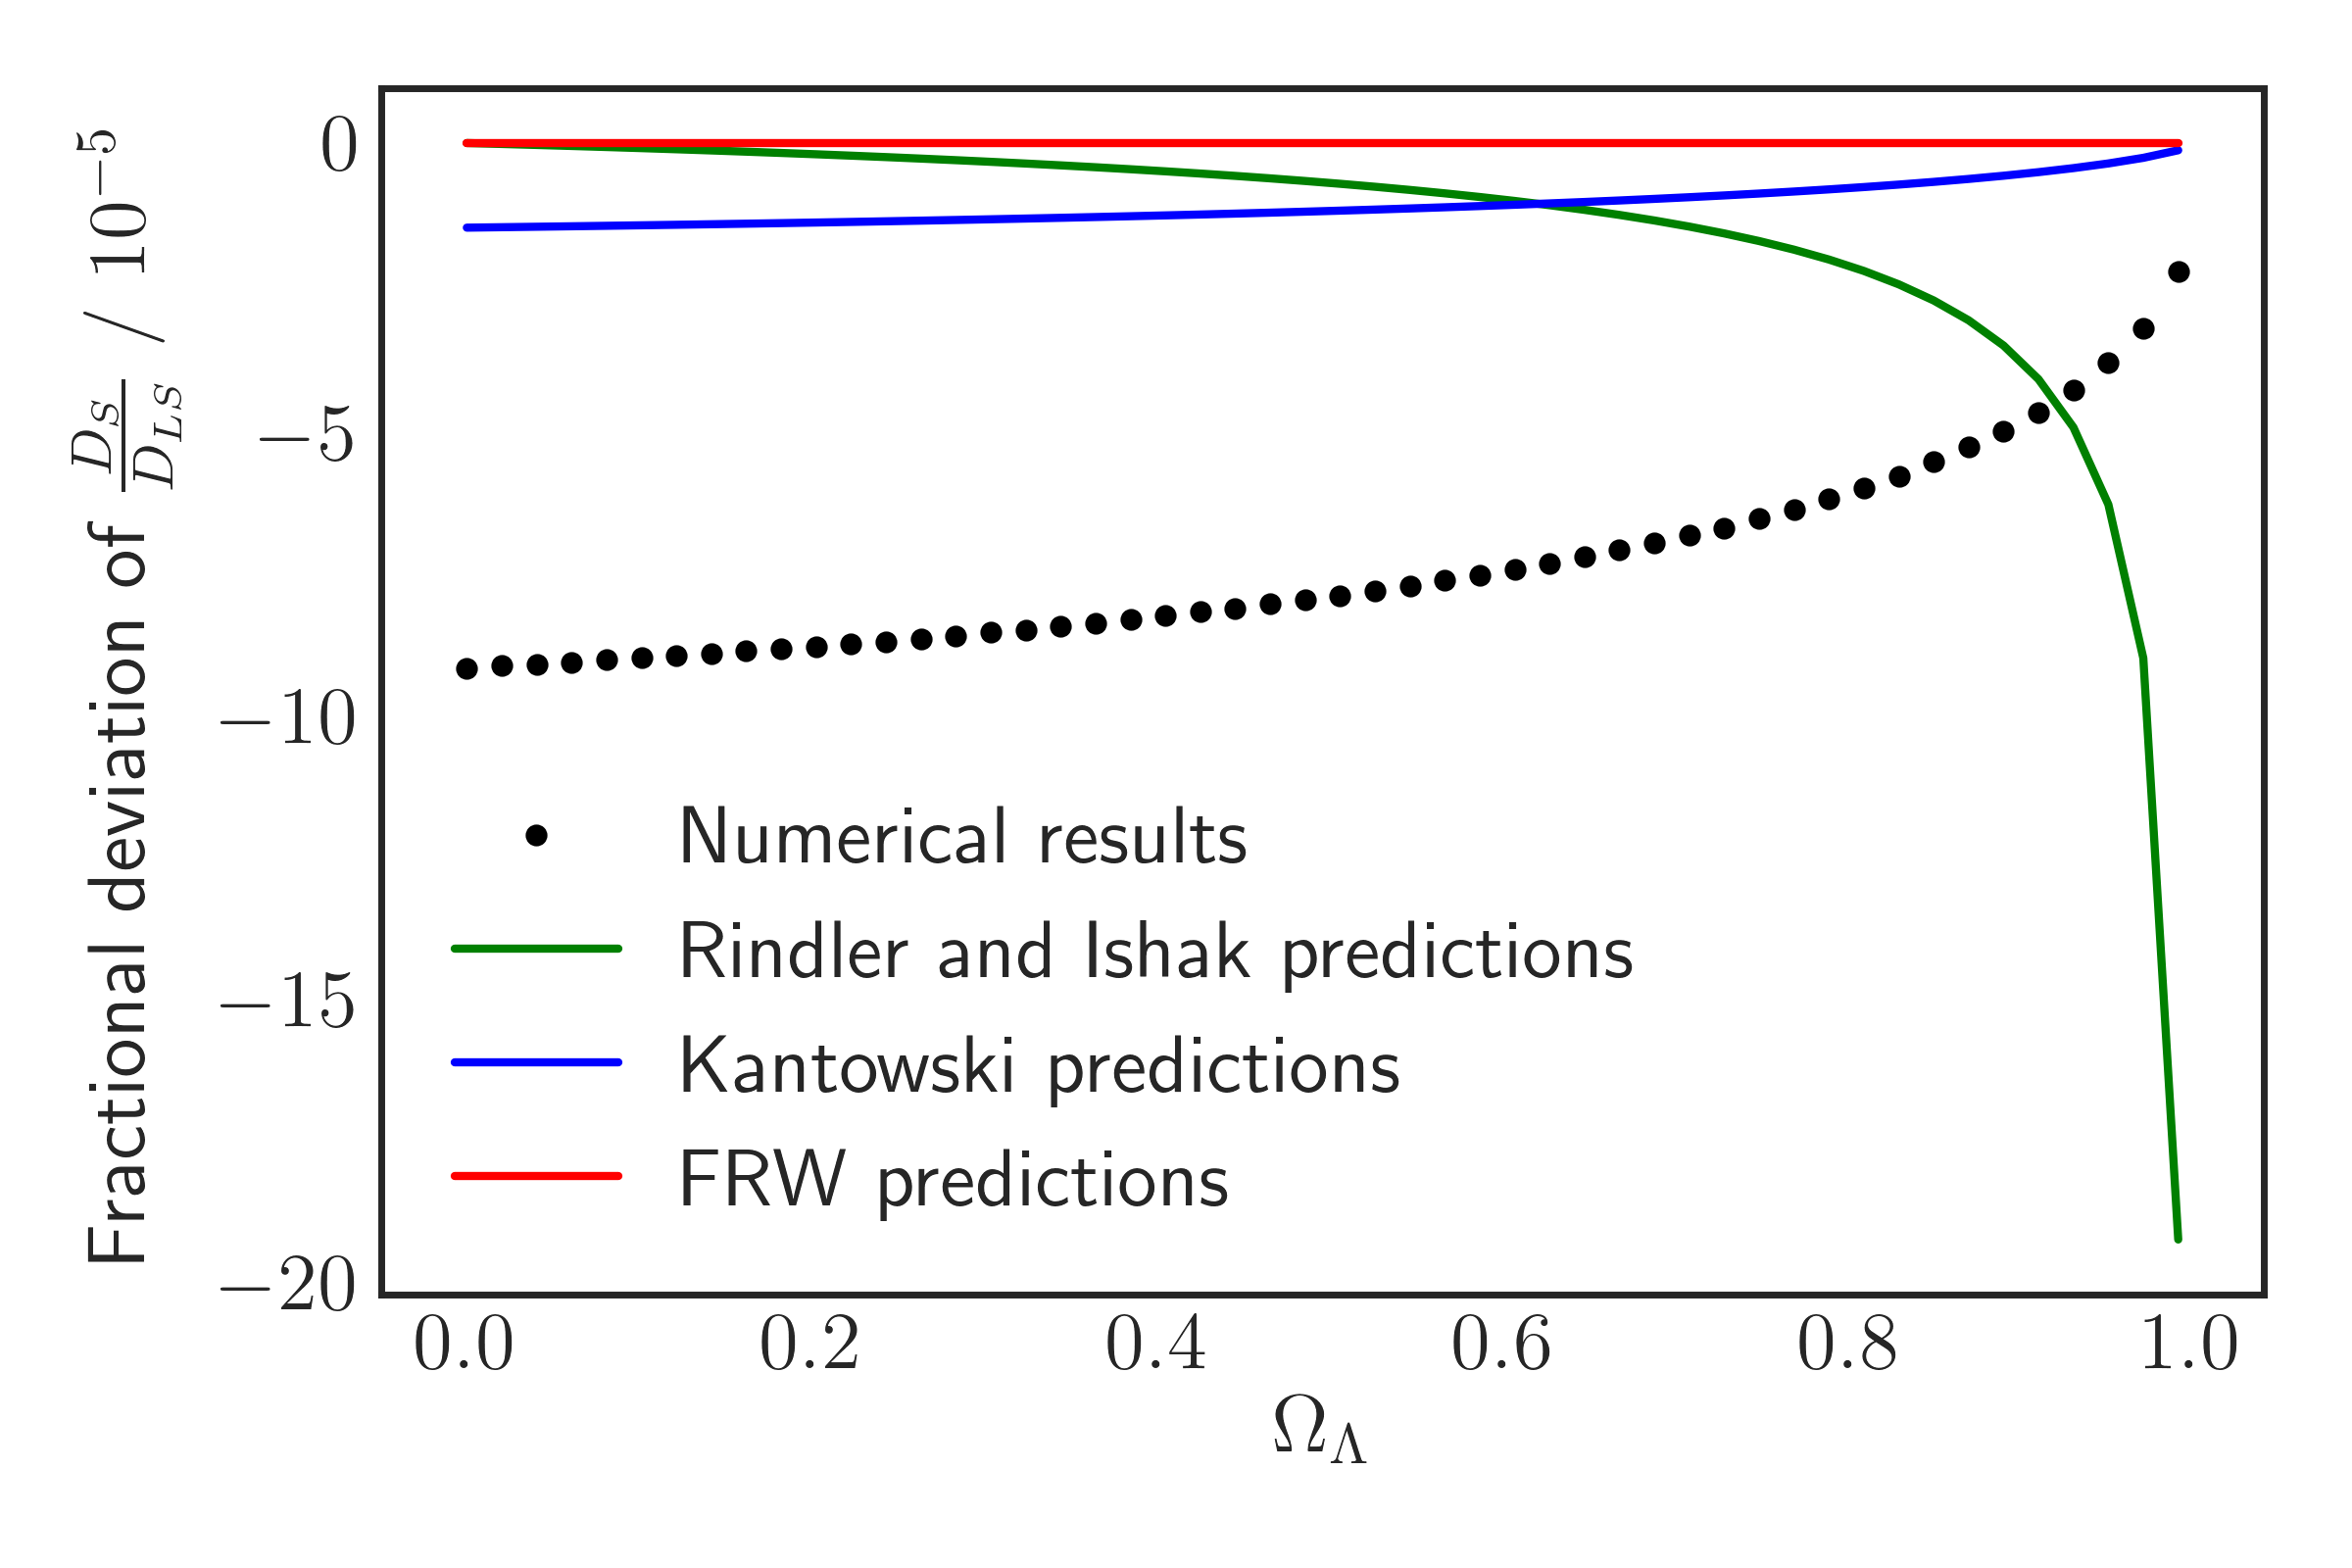
\includegraphics[height=0.5\linewidth]{images/ltb.png}
  \caption{Results for the LTB model with parameters $c = 10$, $M_{\text{total}} = 10^{12} M_\odot$, $\theta_E = 0.5^{\prime\prime}$, $R_{\text{max}} = r_h/2$, $R_{\text{vir}} = r_h/100$. Numerical results are plotted as a fractional deviation from the conventional FRW lensing predictions, as are the Rindler \& Ishak and Kantowski predictions. }
  \label{fig:ltb-results}
\end{figure}

The results show the same general trend as the Kottler case, except now the there is a bigger discrepancy between the conventional result and the numerical result. This is likely the error induced by the thin-screen approximation. \citet{frittelli2011accuracy} found that the thin lens approximation when applied to the NFW mass profile produced an error of similar magnitude. 

% This ensures that the subsequent sections are being included as root
% items in the bookmark structure of your PDF reader.
\bookmarksetup{startatroot}
\backmatter

  \printindex
  \printbibliography[title={References},heading=bibintoc]

\end{document}